\subsection{} 

Fig.~\ref{fig:fmkeypoints} shows the 20 matching image points using mouse-clicking as done in HW3 previously. These coordinates were saved and submitted with the submitted assignment files named {\it FM\_1.txt} and {\it FM\_2.txt}. 

\begin{figure}[ht]
\centering
	\begin{subfigure}{0.5\textwidth}
    {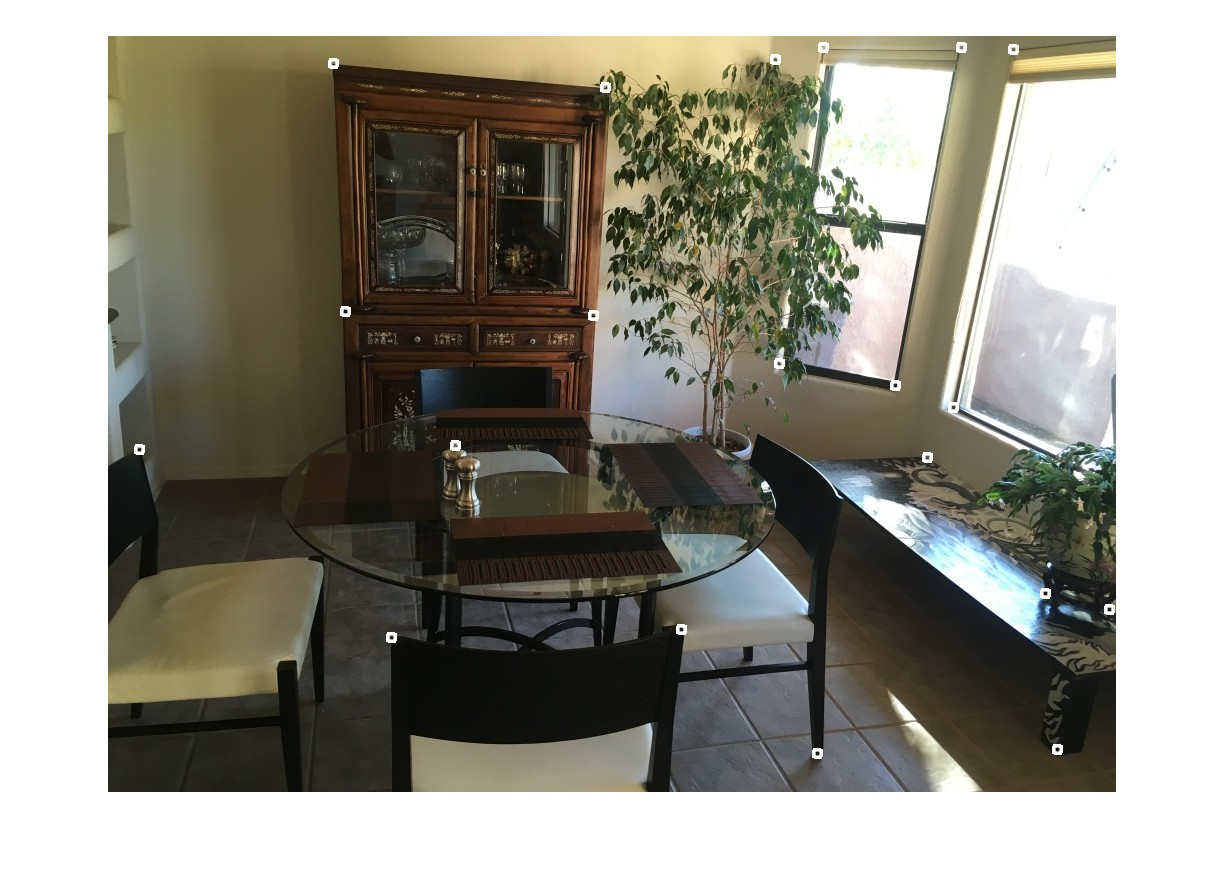
\includegraphics[width=3in]{new_figs/fm1_kp.jpg}}
	\caption{20 keypoints for scene 1}
	\end{subfigure}
	\begin{subfigure}{0.5\textwidth}
    {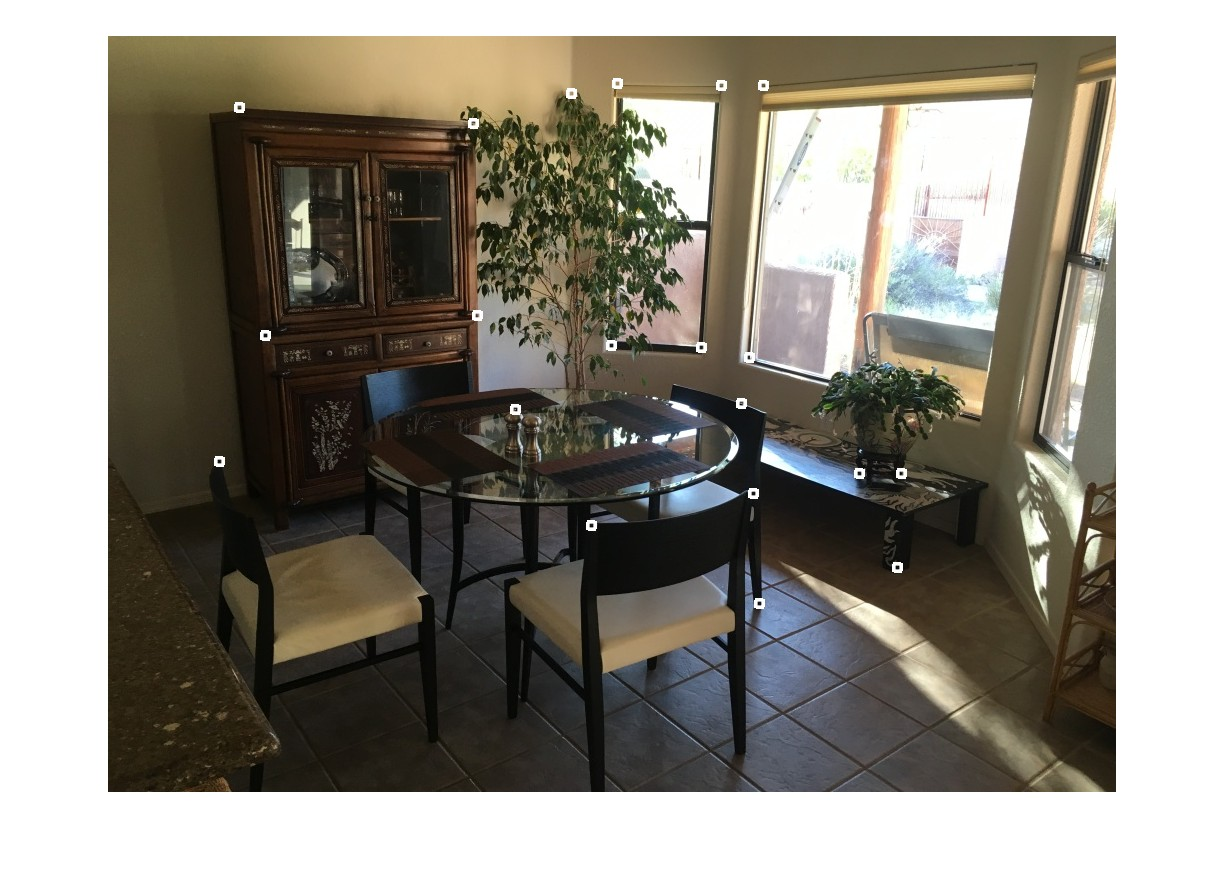
\includegraphics[width=3in]{new_figs/fm2_kp.jpg}
	\caption{20 keypoints for scene 2}
	\end{subfigure}
	\caption{Figure showing matches across two arbitrary views of the same scene. The image points were chosen carefully such that the points occur in both scence.}
\label{fig:fmkeypoints}
\end{figure}


\subsection{} 

Using the fact that $(x')^T F x = 0$ everytime, we can compute the fundamental matrix in the following way. Let:
\begin{equation*}
{\mathbf X'} = 
\begin{bmatrix}
x' \\
y' \\
1
\end{bmatrix},
\quad
{\mathbf X} = 
\begin{bmatrix}
x \\
y \\
1
\end{bmatrix},
\quad
{\mathbf F} = 
\begin{bmatrix}
F_{11} & F_{12} & F_{13}\\
F_{21} & F_{22} & F_{23}\\
F_{31} & F_{32} & F_{33}
\end{bmatrix},
\end{equation*}

Then we have:
\begin{equation*}
\begin{bmatrix}
x' & y' & 1 \\
\end{bmatrix} 
\begin{bmatrix}
F_{11} & F_{12} & F_{13}\\
F_{21} & F_{22} & F_{23}\\
F_{31} & F_{32} & F_{33}
\end{bmatrix}
\begin{bmatrix}
x \\
y \\
1
\end{bmatrix}
= 0
\end{equation*}

\begin{equation*}
\implies
\begin{bmatrix}
x'F_{11} + y'F_{21} + F_{31} & x'F_{12} + y'F_{22} + F_{32} & x'F_{13} + y'F_{23} + F_{33}
\end{bmatrix}
\begin{bmatrix}
x \\
y \\
1
\end{bmatrix}
 = 0
\end{equation*}

Let ${\mathbf F_i}$ be the row vectors of the matrix $F$ for $i = \{1, 2, 3\}$.
\begin{equation*}
\implies
\begin{bmatrix}
\begin{bmatrix}
x' & y' & 1 \\
\end{bmatrix} \cdot {\mathbf F_1}^T

&

\begin{bmatrix}
x' & y' & 1 \\
\end{bmatrix} \cdot {\mathbf F_2}^T

& 

\begin{bmatrix}
x' & y' & 1 \\
\end{bmatrix} \cdot {\mathbf F_3}^T

\end{bmatrix}
\begin{bmatrix}
x \\
y \\
1
\end{bmatrix}
 = 0
\end{equation*}


Therefore, we have:
\begin{equation*}
\begin{bmatrix}
x'x & y'x & x & x'y & y'y & y & x' & y' & 1 
\end{bmatrix} 
\begin{bmatrix}
F_{11} \\
F_{12} \\
F_{13} \\
F_{21} \\
F_{22} \\
F_{23} \\
F_{31} \\
F_{32} \\
F_{33}
\end{bmatrix}
= 0,
\end{equation*}

which we can solve using homogenous least squares method for any number of points ${\mathbf X}$ and corresponding ${\mathbf X'}$. 

\subsection{} 
Using the derivation in Part 5.2, we find $F$ using the 12 (training) coordinates collected in Part 5.1. We tested the computed $F$ on the other $8$ coordinates and yielded an RMS of $0.0249$. 

\subsection{}
Using the given image-pairs and the clicked point-pairs, for this part we used the derived $F$ to draw the epipolar line on both images for each point in the other image. Fig.~\ref{fig:mirrors} shows these lines together with the marked points. On observation, it looks like that the epipolar lines help determine the position of the camera for both scenes! (This question was a lot of fun to tackle.)

\begin{figure}[ht]
\centering
	\begin{subfigure}{0.5\textwidth}
    {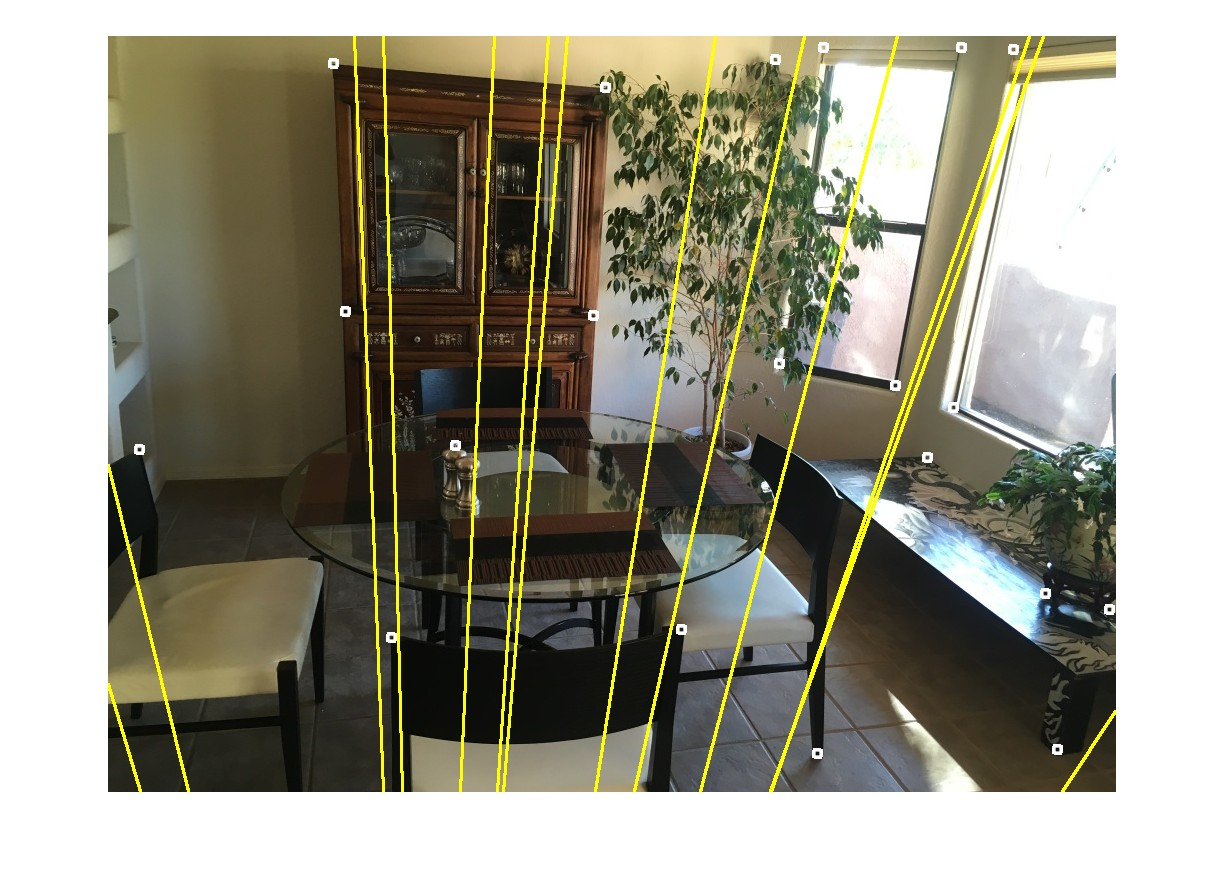
\includegraphics[width=3in]{new_figs/ep1-d1.jpg}}
	\caption{Epipolar lines on scene 1 using points from scene 2}
	\end{subfigure}
	\begin{subfigure}{0.5\textwidth}
    {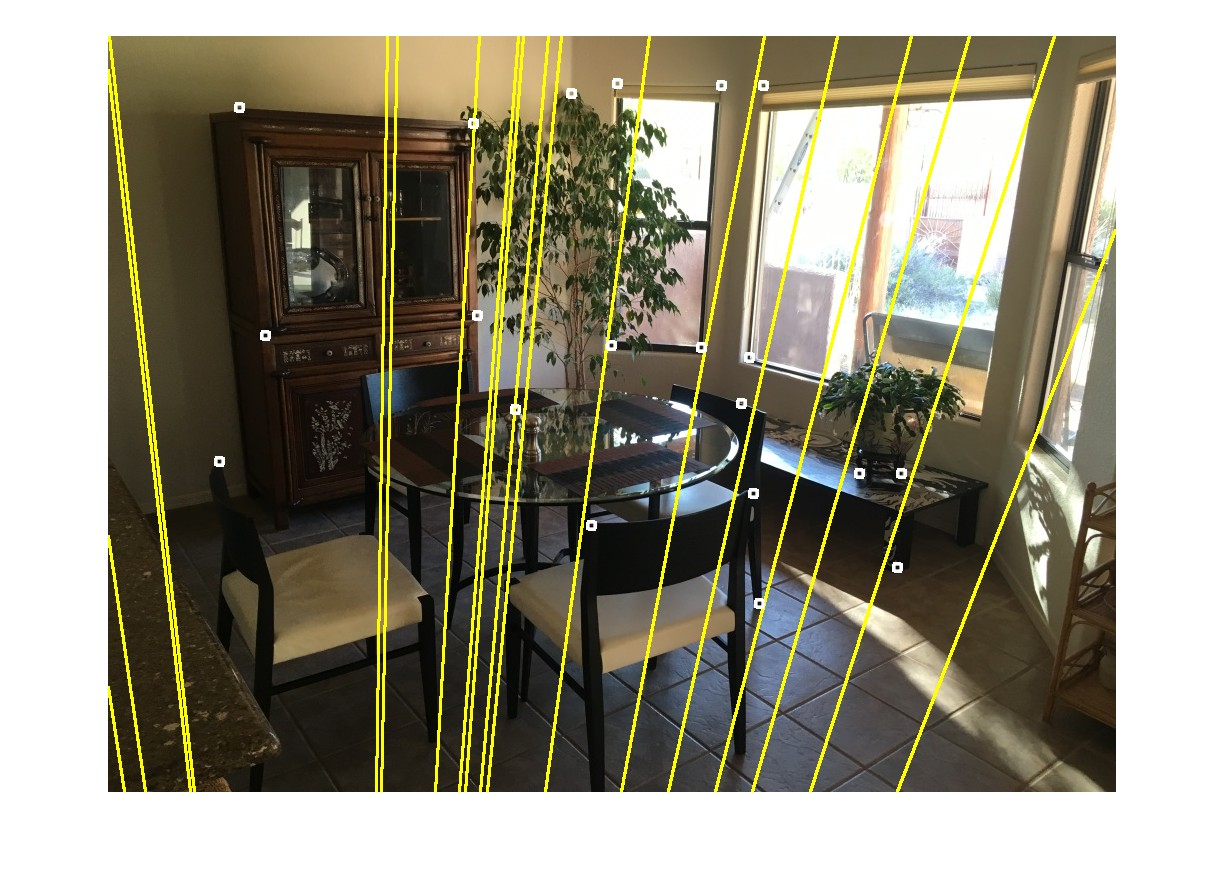
\includegraphics[width=3in]{new_figs/ep2-d1.jpg}
	\caption{Epipolar lines on scene 2 using points from scene 1}
	\end{subfigure}
	\caption{Figure showing epipolar lines on both scences. These were determined by first collecting 20 points by mouse-clicking and then distribution the points into training (of 12 points) and test (of 8 points) sets. Using the training points, we determined the fundamental matrix $F$ using the derivation in 5.2 and used the 8 test points to see how close they are to 0, since $(x')^T F x = 0$ everytime.}
\label{fig:mirrors}
\end{figure}
